\subsubsection{Kruskal (Baseado em DSU e Ordenação de Arestas)}
O algoritmo de Kruskal ordena todas as arestas do grafo em ordem crescente de
peso. Em seguida, itera por cada aresta utilizando uma estrutura de DSU: se os
vértices da aresta pertencem a conjuntos diferentes, nós os unimos e
adicionamos a aresta à MST. Caso contrário, a aresta é descartada para evitar
ciclos. A complexidade de tempo é $\mathcal{O}(E \log E)$ devido à ordenação
das arestas.

\paragraph{Pseudo-Código: }\mbox{}\\
\begin{algorithm}[H]
    \SetAlgoLined
    \SetKwFunction{Kruskal}{Kruskal}
    \SetKwProg{Fn}{Função}{:}{}

    \Fn{\Kruskal{$arestas, V$}}{
        $mst \gets \emptyset$\;
        \text{Ordenar } $arestas$ \text{ em ordem crescente de peso}\;
        \text{Inicializar } $dsu$ \text{ com } $V$ \text{ elementos}\;

        \ParaCada{$(peso, u, v) \in arestas$}{
            \Se{$dsu.find(u) \neq dsu.find(v)$}{
                $dsu.unite(u, v)$\;
                $mst.add((u, v, peso))$\;
            }
        }
        \Retorna $mst$\;
    }
    \caption{Algoritmo de Kruskal}
\end{algorithm}

Veja o Kruskal funcionando, selecionando arestas em ordem crescente de peso sem
formar ciclos:\\ \vspace{0.5cm} \noindent
\begin{minipage}[t]{0.31\textwidth}
    \centering
    \textbf{Passo 1: Arestas Ordenadas}\\
    \vspace{0.2cm}
    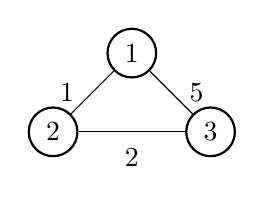
\begin{tikzpicture}[every node/.style={circle, draw, minimum size=0.5cm, thick}]
        \node (1) at (0, 1) {1};
        \node (2) at (-1, 0) {2};
        \node (3) at (1, 0) {3};
        \draw (1) -- node[left, draw=none, fill=none] {1} (2);
        \draw (2) -- node[below, draw=none, fill=none] {2} (3);
        \draw (1) -- node[right, draw=none, fill=none] {5} (3);
    \end{tikzpicture}

    \vspace{0.2cm}
    \footnotesize
    \raggedright
    Arestas ordenadas por peso: (1-2, peso 1), (2-3, peso 2), (1-3, peso 5).
\end{minipage}%
\hfill
%
\begin{minipage}[t]{0.31\textwidth}
    \centering
    \textbf{Passo 2: Adiciona aresta (1-2)}\\
    \vspace{0.2cm}
    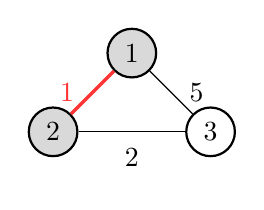
\begin{tikzpicture}[every node/.style={circle, draw, minimum size=0.5cm, thick}]
        \node[fill=gray!30] (1) at (0, 1) {1};
        \node[fill=gray!30] (2) at (-1, 0) {2};
        \node (3) at (1, 0) {3};
        \draw[very thick, red!80] (1) -- node[left, draw=none, fill=none] {1} (2);
        \draw (2) -- node[below, draw=none, fill=none] {2} (3);
        \draw (1) -- node[right, draw=none, fill=none] {5} (3);
    \end{tikzpicture}

    \vspace{0.2cm}
    \footnotesize
    \raggedright
    Menor peso (1). Unimos 1 e 2 via DSU. Aresta aceita na MST.
\end{minipage}%
\hfill
%
\begin{minipage}[t]{0.31\textwidth}
    \centering
    \textbf{Passo 3: Adiciona (2-3)}\\
    \vspace{0.2cm}
    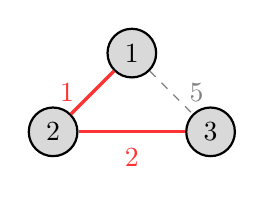
\begin{tikzpicture}[every node/.style={circle, draw, minimum size=0.5cm, thick}]
        \node[fill=gray!30] (1) at (0, 1) {1};
        \node[fill=gray!30] (2) at (-1, 0) {2};
        \node[fill=gray!30] (3) at (1, 0) {3};
        \draw[very thick, red!80] (1) -- node[left, draw=none, fill=none] {1} (2);
        \draw[very thick, red!80] (2) -- node[below, draw=none, fill=none] {2} (3);
        \draw[dashed, gray] (1) -- node[right, draw=none, fill=none] {5} (3);
    \end{tikzpicture}

    \vspace{0.2cm}
    \footnotesize
    \raggedright
    Próxima menor (2). Unimos 2 e 3. Aresta (1-3) é ignorada (formaria ciclo). MST pronta! Custo: 3.
\end{minipage}

\vspace{0.3cm}

\paragraph{Implementação: }\mbox{}\\
\textbf{Python: }
\begin{lstlisting}[language=Python]
def kruskal(n, arestas):
    # arestas = lista de tuplas (peso, u, v)
    arestas.sort()
    dsu = DSU(n)
    mst = []
    custo_total = 0
    
    for peso, u, v in arestas:
        if dsu.unite(u, v):
            mst.append((u, v, peso))
            custo_total += peso
            
    return custo_total, mst
\end{lstlisting}

\vspace{0.3cm}
\textbf{C++:}
\begin{lstlisting}[language=C++]
struct Aresta {
    int u, v, peso;
    bool operator<(const Aresta& outro) const {
        return peso < outro.peso;
    }
};

int kruskal(int n, vector<Aresta>& arestas) {
    sort(arestas.begin(), arestas.end());
    DSU dsu(n);
    int custoTotal = 0;
    
    for (auto& a : arestas) {
        if (dsu.unite(a.u, a.v)) {
            custoTotal += a.peso;
        }
    }
    return custoTotal;
}
\end{lstlisting}
\newpage